% =============================================================================
% Interface Streamlit -- Documentação da UI
% Pode ser incluído via \input{} no relatório principal
% =============================================================================

\section{Interface de avaliação de medidas}\label{sec:interface-ui}

A ferramenta de avaliação de medidas foi implementada como uma aplicação web
interativa utilizando o \emph{framework} Streamlit. O objetivo principal da
interface é permitir que o engenheiro de processo avalie, de forma rápida e
visual, quais grandezas de um modelo de processo são calculáveis a partir de
um conjunto de medidores instalados e, quando necessário, identifique o menor
acréscimo de instrumentação para tornar todas as grandezas calculáveis.

A aplicação está organizada em três abas funcionais, um painel lateral de
configuração e uma área de resultados com indicadores-chave de desempenho
(KPIs) e tabelas detalhadas. As subseções a seguir descrevem cada componente
da interface, acompanhadas de capturas de tela representativas.


% ---------------------------------------------------------------------------
\subsection{Visão geral e navegação}\label{ssec:ui-visao-geral}

Ao acessar a aplicação, o usuário é apresentado à tela inicial ilustrada na
Figura~\ref{fig:ui-visao-geral}. O título ``Avaliação de medidas do
processo'' sintetiza o propósito da ferramenta. Logo abaixo, um alerta
informativo (caixa verde) exibe o critério de sucesso adotado: todas as
grandezas do modelo devem passar a ser calculáveis com as medidas escolhidas.
Esse critério é compartilhado pelas abas de classificação e de instrumentação
mínima.

A navegação é feita por meio de três abas:

\begin{enumerate}[label=\arabic*.]
  \item \textbf{Classificação} --- Avalia o que o processo consegue calcular
        hoje, dada a lista de medidores já instalados, sem propor nenhuma
        alteração.
  \item \textbf{Inst.\ mínima} --- Encontra o menor acréscimo de medidores
        para calcular tudo. Por padrão, a busca é \emph{automática}; no
        preset de candidatos restritos ou no YAML avançado, o usuário pode
        restringir os candidatos (por exemplo, sensores falhos).
  \item \textbf{Regras MILP (URS)} --- Otimização pelas regras de engenharia
        do modelo URS ($F+R$, permeados, limites por equação). Utiliza um
        critério diferente da análise estrutural das abas anteriores.
\end{enumerate}

Um seletor de \textbf{cenário} permite escolher entre configurações
pré-definidas (presets). Cada preset carrega automaticamente o arquivo YAML
correspondente, incluindo o perfil de equações, a lista de medidores e o
objetivo de análise.

\begin{figure}[htbp]
  \centering
  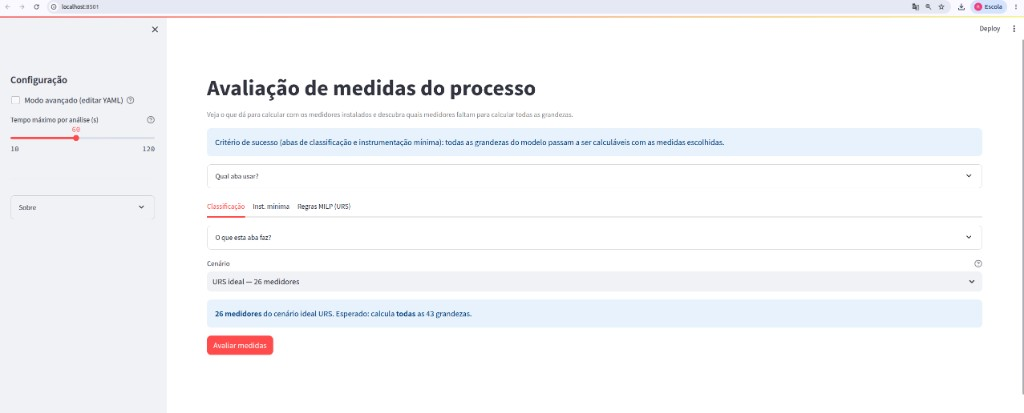
\includegraphics[width=0.95\textwidth]{figures/fig_ui_visao_geral}
  \caption{Tela inicial da aplicação: título, critério de sucesso, abas de
           navegação, seletor de cenário e botão ``Avaliar medidas''.}
  \label{fig:ui-visao-geral}
\end{figure}


% ---------------------------------------------------------------------------
\subsection{Modo avançado e guia de abas}\label{ssec:ui-modo-avancado}

O painel lateral (\emph{sidebar}) oferece duas opções de configuração:

\begin{itemize}
  \item \textbf{Modo avançado (editar YAML)} --- Quando ativado, exibe o
        editor YAML \emph{inline} e o \emph{uploader} de arquivos,
        permitindo que o usuário modifique diretamente os parâmetros do
        cenário ou carregue um arquivo YAML personalizado.
  \item \textbf{Tempo máximo por análise (s)} --- Controle deslizante que
        define o limite de tempo (em segundos) para o \emph{solver} CP-SAT
        ou MILP, com faixa de 16 a 120\,s.
\end{itemize}

A Figura~\ref{fig:ui-modo-avancado} mostra a interface com o modo avançado
ativado. Observa-se o \emph{expander} ``Qual aba usar?'' aberto, que fornece
uma descrição resumida de cada aba para orientar o usuário. Logo abaixo,
aparece a área de \emph{upload} de arquivo YAML e a descrição do cenário
selecionado (``26 medidores do cenário ideal URS. Esperado: calcula
\textbf{todas} as 43 grandezas.'').

\begin{figure}[htbp]
  \centering
  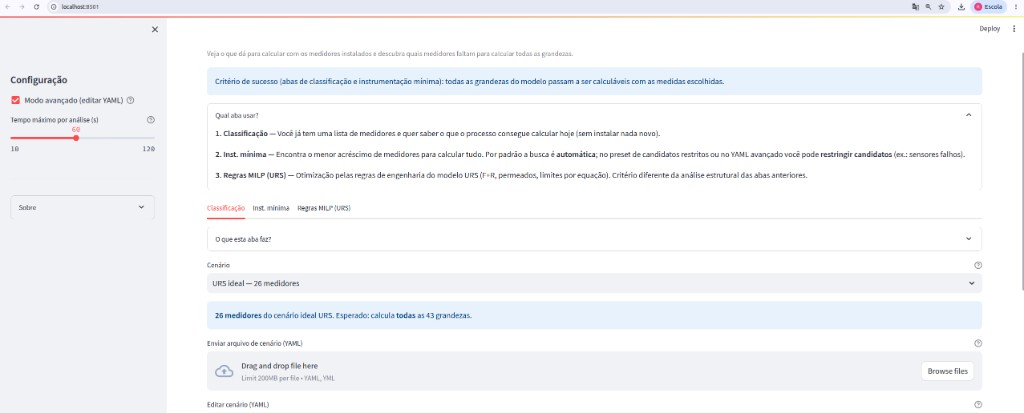
\includegraphics[width=0.95\textwidth]{figures/fig_ui_modo_avancado}
  \caption{Modo avançado ativado: expander ``Qual aba usar?'' com descrição
           das três abas, área de upload e descrição do cenário.}
  \label{fig:ui-modo-avancado}
\end{figure}


% ---------------------------------------------------------------------------
\subsection{Editor YAML e upload de cenários}\label{ssec:ui-editor-yaml}

Quando o modo avançado está ativo, um editor de texto integrado permite
visualizar e editar o conteúdo YAML do cenário carregado
(Figura~\ref{fig:ui-editor-yaml}). O formato YAML segue o esquema definido
pelo pacote \texttt{structural\_obs}, contendo os seguintes campos
principais:

\begin{itemize}
  \item \texttt{schema\_version} --- Versão do esquema (atualmente
        \texttt{"1.0"}).
  \item \texttt{case.id} --- Identificador único do caso.
  \item \texttt{case.name} --- Nome descritivo do cenário.
  \item \texttt{case.equations\_profile} --- Perfil de equações do modelo de
        processo (e.g.\ \texttt{urs\_document}).
  \item \texttt{case.instrumentation.measured} --- Lista das grandezas já
        medidas (medidores instalados).
  \item \texttt{case.instrumentation.known\_constants} --- Constantes
        conhecidas do processo.
  \item \texttt{case.analysis.objective} --- Objetivo da análise
        (\texttt{classify}, \texttt{min\_placement} ou
        \texttt{milp\_verify}).
\end{itemize}

O usuário pode também arrastar e soltar (\emph{drag and drop}) um arquivo
\texttt{.yaml} ou \texttt{.yml} diretamente na área de upload, substituindo
o cenário atual.

\begin{figure}[htbp]
  \centering
  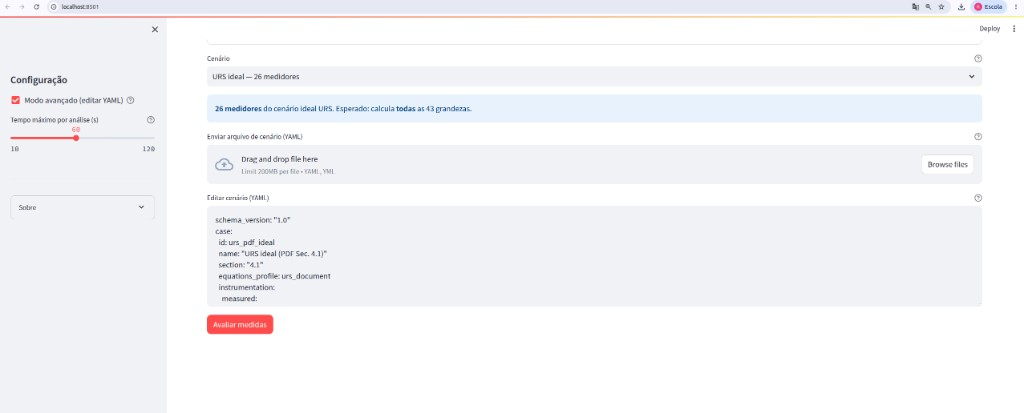
\includegraphics[width=0.95\textwidth]{figures/fig_ui_editor_yaml}
  \caption{Editor YAML integrado: o usuário pode modificar diretamente os
           parâmetros do cenário ou enviar um arquivo externo.}
  \label{fig:ui-editor-yaml}
\end{figure}


% ---------------------------------------------------------------------------
\subsection{Resultados: indicadores-chave (KPIs)}\label{ssec:ui-kpis}

Após clicar no botão ``Avaliar medidas'', a aplicação executa o modelo
CP-SAT e apresenta o resultado em dois níveis: um painel de KPIs e uma
tabela detalhada de grandezas. A Figura~\ref{fig:ui-kpis} ilustra o painel
de KPIs para o cenário ideal URS com 26 medidores. Os indicadores exibidos
são:

\begin{itemize}
  \item \textbf{Calculável hoje} --- Número de grandezas que o modelo
        consegue determinar com a instrumentação atual (medidas diretas mais
        inferidas). No exemplo, 43 de 43.
  \item \textbf{Calculadas (inferidas)} --- Grandezas não medidas
        diretamente, mas calculáveis a partir dos balanços. No exemplo, 17.
  \item \textbf{Indetermináveis} --- Grandezas que não podem ser calculadas
        com a instrumentação atual. No exemplo, 0.
  \item \textbf{Medidores instalados} --- Quantidade total de medidores no
        cenário. No exemplo, 26.
  \item \textbf{Ainda não calculável} --- Grandezas sem cobertura, mesmo
        considerando inferência indireta. No exemplo, 0.
  \item \textbf{Pontos abertos} --- Tears abertos ($\mathit{tear\_open}$):
        pontos de ruptura no grafo bipartido onde o balanço não pode ser
        resolvido sem medida adicional. No exemplo, 0.
  \item \textbf{Alcance com pontos críticos} --- Cobertura externa
        ($C_{\text{ext}}$): grandezas atingíveis considerando dependência de
        tears abertos. No exemplo, 43 de 43.
  \item \textbf{Cobertura direta} --- Cobertura direta
        ($C_{\text{dir}}$): grandezas emparelhadas diretamente, sem
        dependência de tears. No exemplo, 43 de 43.
\end{itemize}

Abaixo dos KPIs, a seção ``Todas as grandezas do modelo'' lista cada
variável com sua situação (``já medido'', ``calculado direto'',
``indeterminável'' etc.), permitindo inspeção individual.

\begin{figure}[htbp]
  \centering
  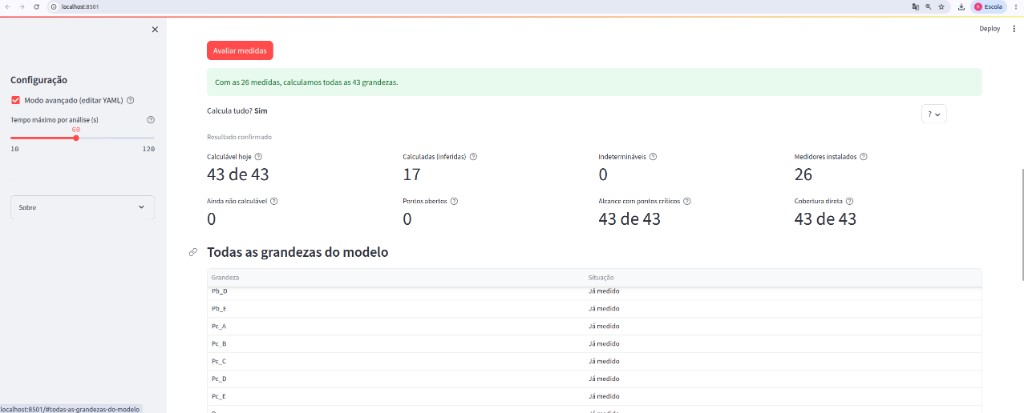
\includegraphics[width=0.95\textwidth]{figures/fig_ui_resultado_kpis}
  \caption{Painel de KPIs após avaliação: métricas de cobertura,
           inferência, instrumentação e tabela de grandezas.}
  \label{fig:ui-kpis}
\end{figure}


% ---------------------------------------------------------------------------
\subsection{Detalhamento por situação e métricas técnicas}%
\label{ssec:ui-detalhes-tecnicos}

A Figura~\ref{fig:ui-detalhes-tecnicos} apresenta a seção de detalhamento,
acessível por \emph{scroll} abaixo dos KPIs. Essa seção é composta por:

\paragraph{Detalhamento por situação.}
Dois \emph{expanders} filtram as grandezas por categoria:
\begin{itemize}
  \item \textbf{Já medido} --- Lista as 26 grandezas com medidores
        instalados (e.g.\ $P_{a,A}$, $P_{b,B}$, $R_{c,C}$, $R_{a,A}$
        etc.).
  \item \textbf{Calculado direto} --- Lista as 11 grandezas inferidas
        diretamente por emparelhamento nos balanços (e.g.\ $F$, $F_A$,
        $F_B$, $P_A$, $R_{b,A}$ etc.).
\end{itemize}
Adicionalmente, as listas de \textbf{grandezas indetermináveis} e
\textbf{pontos em que o balanço ficou aberto} são exibidas (ambas vazias no
cenário ideal).

\paragraph{Detalhes técnicos.}
Um painel de métricas resume o resultado do \emph{solver}:
\begin{itemize}
  \item $C_{\text{cl}}$ (cobertura fechada) --- 43/43.
  \item $C_{\text{ext}}$ (alcance externo) --- 43/43.
  \item $C_{\text{dir}}$ (cobertura direta) --- 43/43.
  \item \textbf{Status do solver} --- \texttt{OPTIMAL}.
  \item \textbf{Tears abertos} --- 0.
  \item \textbf{Indetermináveis efetivas} --- 0.
  \item \textbf{Equações no modelo} --- 19.
\end{itemize}

O botão ``Baixar relatório completo (ZIP)'' permite exportar todos os dados
da análise em formato estruturado para documentação ou auditoria.

\begin{figure}[htbp]
  \centering
  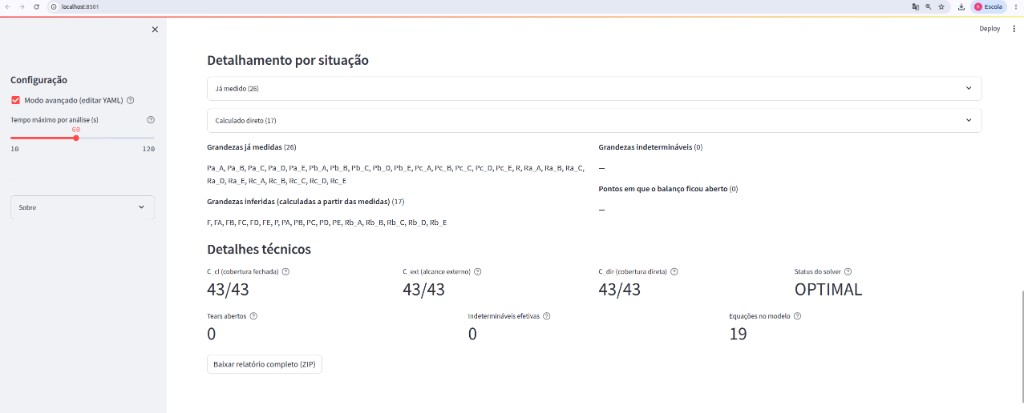
\includegraphics[width=0.95\textwidth]{figures/fig_ui_detalhes_tecnicos}
  \caption{Detalhamento por situação (expanders), listas de grandezas e
           painel de métricas técnicas com status do solver.}
  \label{fig:ui-detalhes-tecnicos}
\end{figure}


% ---------------------------------------------------------------------------
\subsection{Fluxo de uso típico}\label{ssec:ui-fluxo}

O fluxo de uso recomendado para o engenheiro de processo é:

\begin{enumerate}[label=\textbf{\arabic*.}]
  \item \textbf{Selecionar um cenário} via o seletor de presets ou carregar
        um arquivo YAML personalizado.
  \item \textbf{Escolher a aba} apropriada:
        \begin{itemize}
          \item \emph{Classificação} para diagnóstico inicial (``o que
                consigo calcular hoje?'').
          \item \emph{Inst.\ mínima} para otimização de instrumentação
                (``quantos medidores preciso acrescentar?'').
          \item \emph{Regras MILP (URS)} para validação contra regras de
                engenharia específicas do modelo URS.
        \end{itemize}
  \item \textbf{Clicar em ``Avaliar medidas''} para executar a análise.
  \item \textbf{Interpretar os KPIs}: verificar se ``Calculável hoje''
        atinge o total de grandezas e se ``Pontos abertos'' é zero.
  \item \textbf{Inspecionar detalhes}: expandir as categorias de situação,
        verificar a lista de grandezas inferidas e os detalhes técnicos do
        solver.
  \item \textbf{Exportar o relatório} (ZIP) para documentação formal, se
        necessário.
\end{enumerate}

Para cenários mais complexos, o modo avançado permite ajustar manualmente o
YAML --- por exemplo, remover um medidor para simular uma falha de sensor e
avaliar o impacto na observabilidade do processo.
